\section{Object Oriented Design in UML}
\dfn{Object Oriented Design}{
    Object Oriented Design is the phase of software development that follow Object-Oriented Analysis (OOA), where the abstract models of the system are refined and elaborated into detailed specifications that can be directly implemented in an object-oriented programming language
}
\begin{center}
    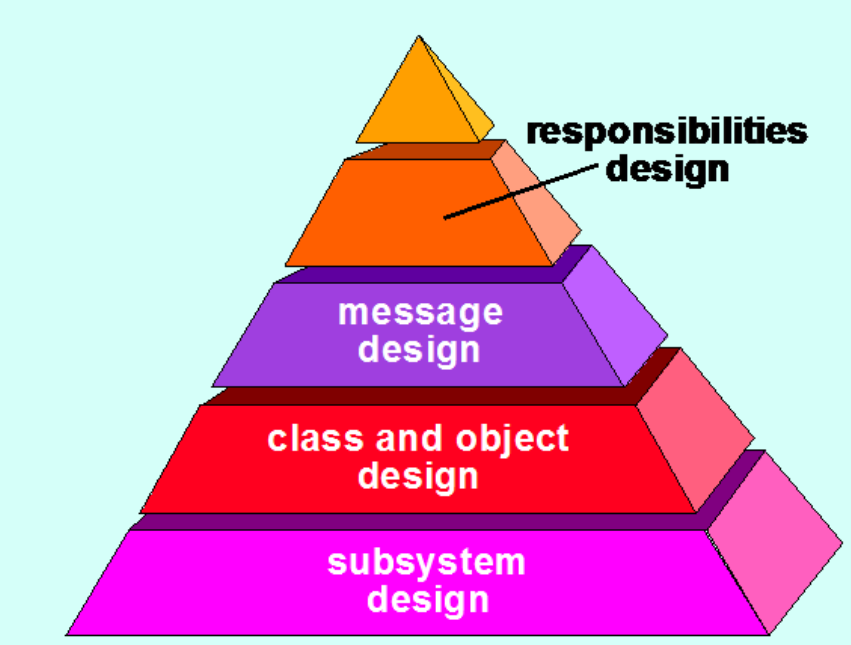
\includegraphics[width=10cm]{piramid_design.png}
\end{center}

In other words the OOD transform the "what" of OOA into the "how", adding technical details necessary for construction while preserving system correctness and maintainability

\subsection{Design Issues}
\begin{itemize}
    \item \textbf{Decomposability}: The facility with which a design method helps the designer decompose a large problem into sub-problems that are easier to solve
    \item \textbf{Composability}: the degree to which a design method ensures that program components (modules), once designed and built, can be reused to create other systems
    \item \textbf{understandability}: the ease with which a program component can be understood without reference to other information or other modules
    \item \textbf{Continuity}: the ability to make small changes in a program and have these changes manifest themselves with corresponding changes in just one or a very few modules
    \item \textbf{protection}: a architectural characteristic that will reduce the propagation of side affects if an error does occur in a given module
\end{itemize}

\subsection{The four pilars for OOD}

These are four components from the complete architecture of any well-designed OO sysyem:
\begin{itemize}
    \item \textbf{Problem domain component}:the subsystems that are
responsible for implementing customer requirements
directly
    \item \textbf{Human interaction component}:the subsystems that implement the user interface (this included reusable GUI subsystems)
    \item \textbf{Task Management Component}: the subsystems that are responsible for controlling and coordinating concurrent tasks that may be packaged within a subsystem or among different subsystems;
    \item \textbf{Data management component}: the subsystem that is responsible for the storage and retrieval of objects.
\end{itemize}

\subsection{OOA vs OOD}
\textbf{Core concept}: OOD refines the abstract OOA model into a concrete, implementable design

\begin{center}
    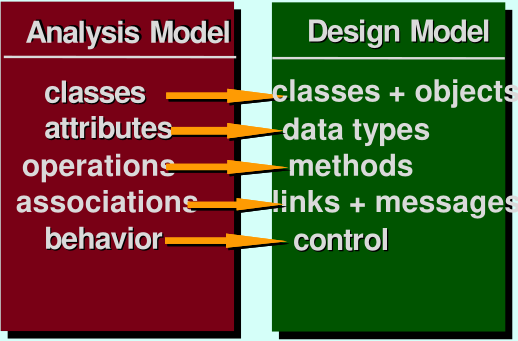
\includegraphics[width=10cm]{ship_btween_OOA_and_OOD.png}
\end{center}
what distinguishes OOD from OOA is:
\begin{itemize}
    \item LEvel of detail:
    \begin{itemize}
        \item Names are fixed
        \item Fixed signatures for messages
        \item Multiplicity \& its realization
        \item Visibility
        \item Algorithms for methods
        \item More detailed sequence/collaboration diagrams
    \end{itemize}
    \item Additional diagram notations
    
    In OOD we have class diagrams, but they refined to match the design of the sysyem.  In addition to class diagrams, we have several other diagrams:

    \begin{itemize}
        \item \textbf{Structural Diagrams}
        \item \textbf{Behavioral Diagrams}
    \end{itemize}
\end{itemize}
\subsection{Structural Diagrams for OOD in UML}
In OOD there are two Structural diagrams:
\begin{itemize}
    \item \textbf{Class Diagrams}: Their structure is the same as for OOA
    \item \textbf{Object Diagrams}:
    \begin{itemize}
        \item They deal with objects, instances of classes
        \item  They are absolutely equivalent to class diagrams
        \item  Given this, we will not analyze them in deep
    \end{itemize} 
\end{itemize}

\subsection{Behavioral Diagrams for OOD in UML}
We'll study:
\begin{itemize}
    \item \textbf{Sequence Diagrams}: Describe the interactions between objects by time ordering
    \item \textbf{Collaboration Diagrams}: Describe the interactions between the objects by organizations
\end{itemize}


\subsubsection{Human interaction component}
the subsystems that implement the user interface (this included reusable GUI subsystems);

In OOD I have class ddiagrams,but they are refined to match the design

\subsection{Statechar diagrams vs interaction diagrams}
\begin{itemize}
    \item \textbf{interaction diagrams}: show how obj interact
\end{itemize}

\subsubsection{Object state}
\dfn{Object state}{
    We define an \textit{Object state} the set of value that describe an obj at a specific moment. State is determinated based on the attribute values
}

\subsection{Interaction Diagrams}
\dfn{
    interaction Diagrams
}{
    Interaction diagrams are behavioral diagrams in UML that model the dynamic aspects of a system by showing how objects collaborate and communicate through message exchanges to accomplish specific tasks or scenarios. They emphasize the flow of control and data between objects during runtime execution
}
\subsubsection{Key charateristic}
\begin{itemize}
    \item Focus on "real" entities (Obj, not classes)
    \item Show msg passing
    \item Can represent both sync and async Communication
    \item Bridge the gap between requirements and implmentation
\end{itemize}

\subsubsection{Two types of implemantion}

Interaction diagrams provide two different perspectives on the same interaction:

\paragraph{Sequence diagrams}
\begin{itemize}
    \item emphasize \textit{when} messagge are sent
    \item Shows object interactions arranged in time sequence
    \item Shows temporal ordering clearly
    \item Best for understanding flow over time
    \item Vertical timeline representation
\end{itemize}

Here we can see timelines:
\begin{center}
    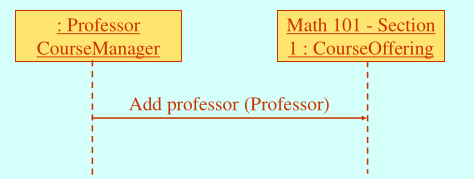
\includegraphics{seq_diagram.png}
\end{center}

\ex{detailed example}{
    \begin{center}
        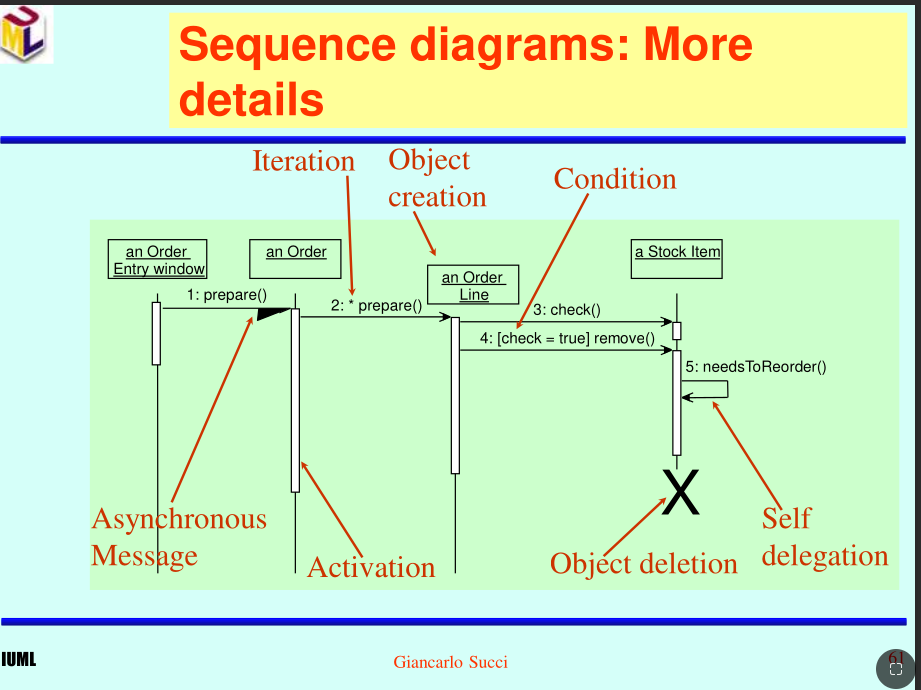
\includegraphics{seq_diag_ex.png}
    \end{center}
}
\subsubsection{Content of sequence diagrams}
We have this content:
\paragraph{objects (participants)}

Lifelines:
\begin{itemize}
    \item Vertical line extending from the obj
    \item represent the obj existence time
    \item contines 'till obj is destroyed
\end{itemize}
\paragraph{Messages} There are two types of msgs:
\begin{itemize}
    \item \textbf{Sysnc msgs}:
    \begin{itemize}
        \item Full arrowhead: $ \longrightarrow $
        \item Caller wait for completion
        \item blocking operation
        \item most common in obj-oriented system
    \end{itemize}
    \item \textbf{Async msgs (signals)}:
    \begin{itemize}
        \item Half arrowhead (stick arrow): $ \rightarrow $
        \item Sender doesn't wait for completion
        \item Non-blocking operation
        \item Used for concurrent operations
    \end{itemize}
    \item \textbf{Return Messages}:
    \begin{itemize}
        \item Typically shown as a dashed arrow: $ \dashrightarrow $
    \end{itemize}
\end{itemize}
